%!TEX root = r-gather.tex

\section{Experimental Results}


We have implemented this distributed algorithm along with the $r$-gather algorithm described in~\cite{Aggarwal06achievinganonymity} to compare their clustering qualities. 
%Both were coded up in Python 2.7.12 using principally, the NetworkX, NumPy, SciPy and Matplotlib packages.

%\subsection{Data Sets}

First, just to have an intuitive understanding of the results in the static setting, what is shown below in Figure~\ref{fig:snapshot} are examples of clusters, for $r=3,5,7,9$  generated by the distributed algorithm on sample point cloud of size $50$. 

%But in the other simulations we used all $9386$ trajectories.
%The points shown are a snapshot of the GPS co-ordinates of 1500 cars driving around Shenzhen city in China.

\begin{figure*}[htpb]
\begin{center}
\begin{tabular}{cc}
\vspace*{-8mm}
	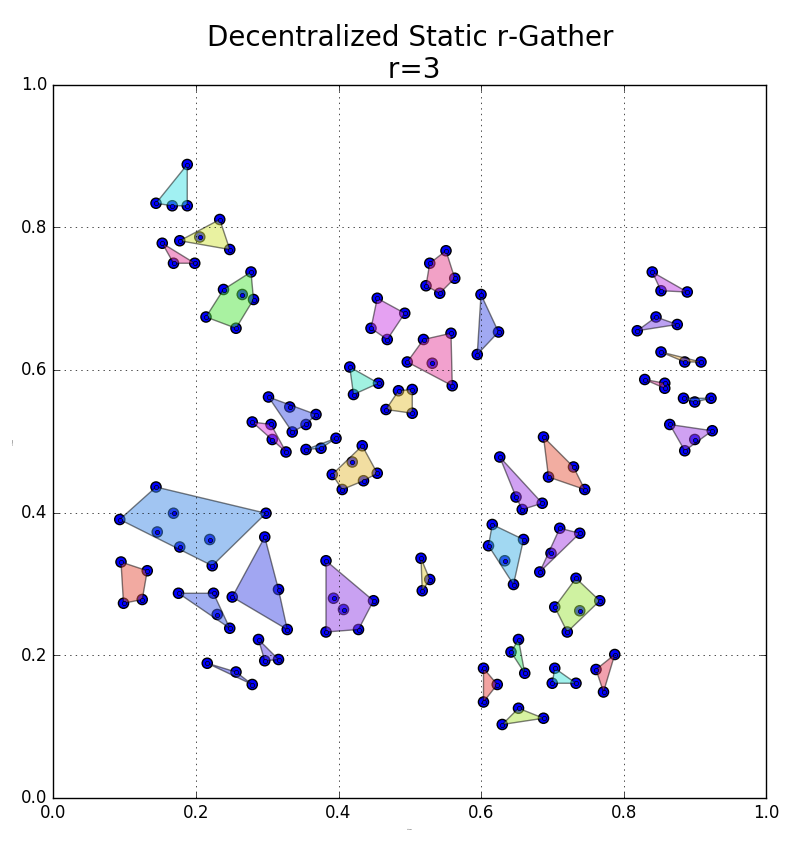
\includegraphics[scale=0.25]{figs/r3.png} &
	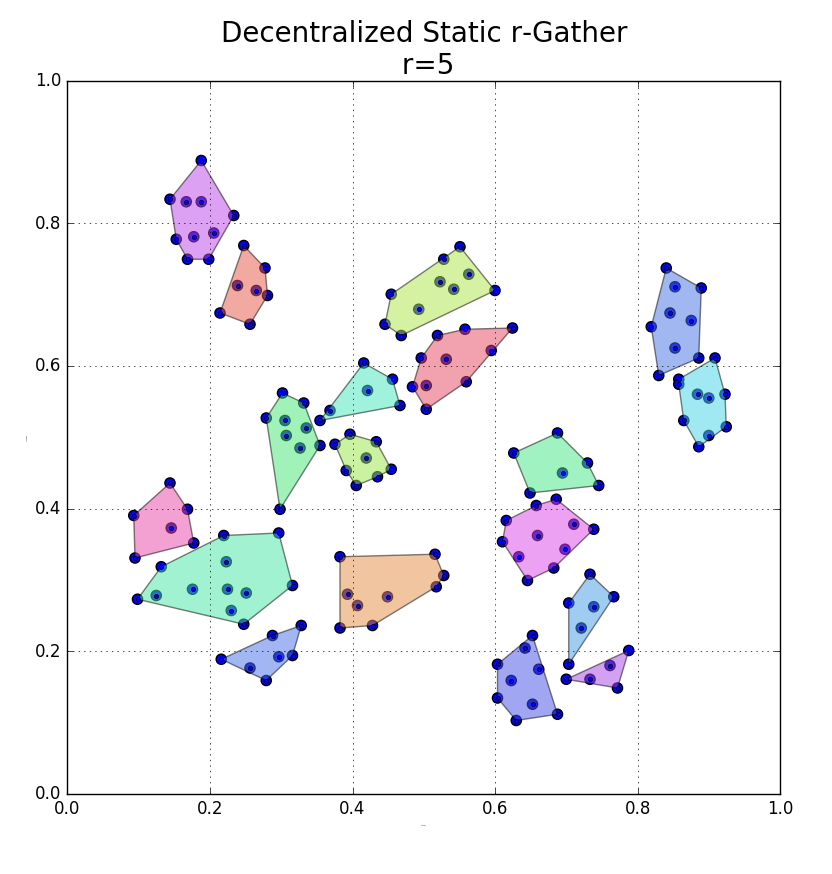
\includegraphics[scale=0.25]{figs/r5.png} \\
\vspace*{-12mm}
%\footnotesize (i) & \footnotesize (ii) \\
	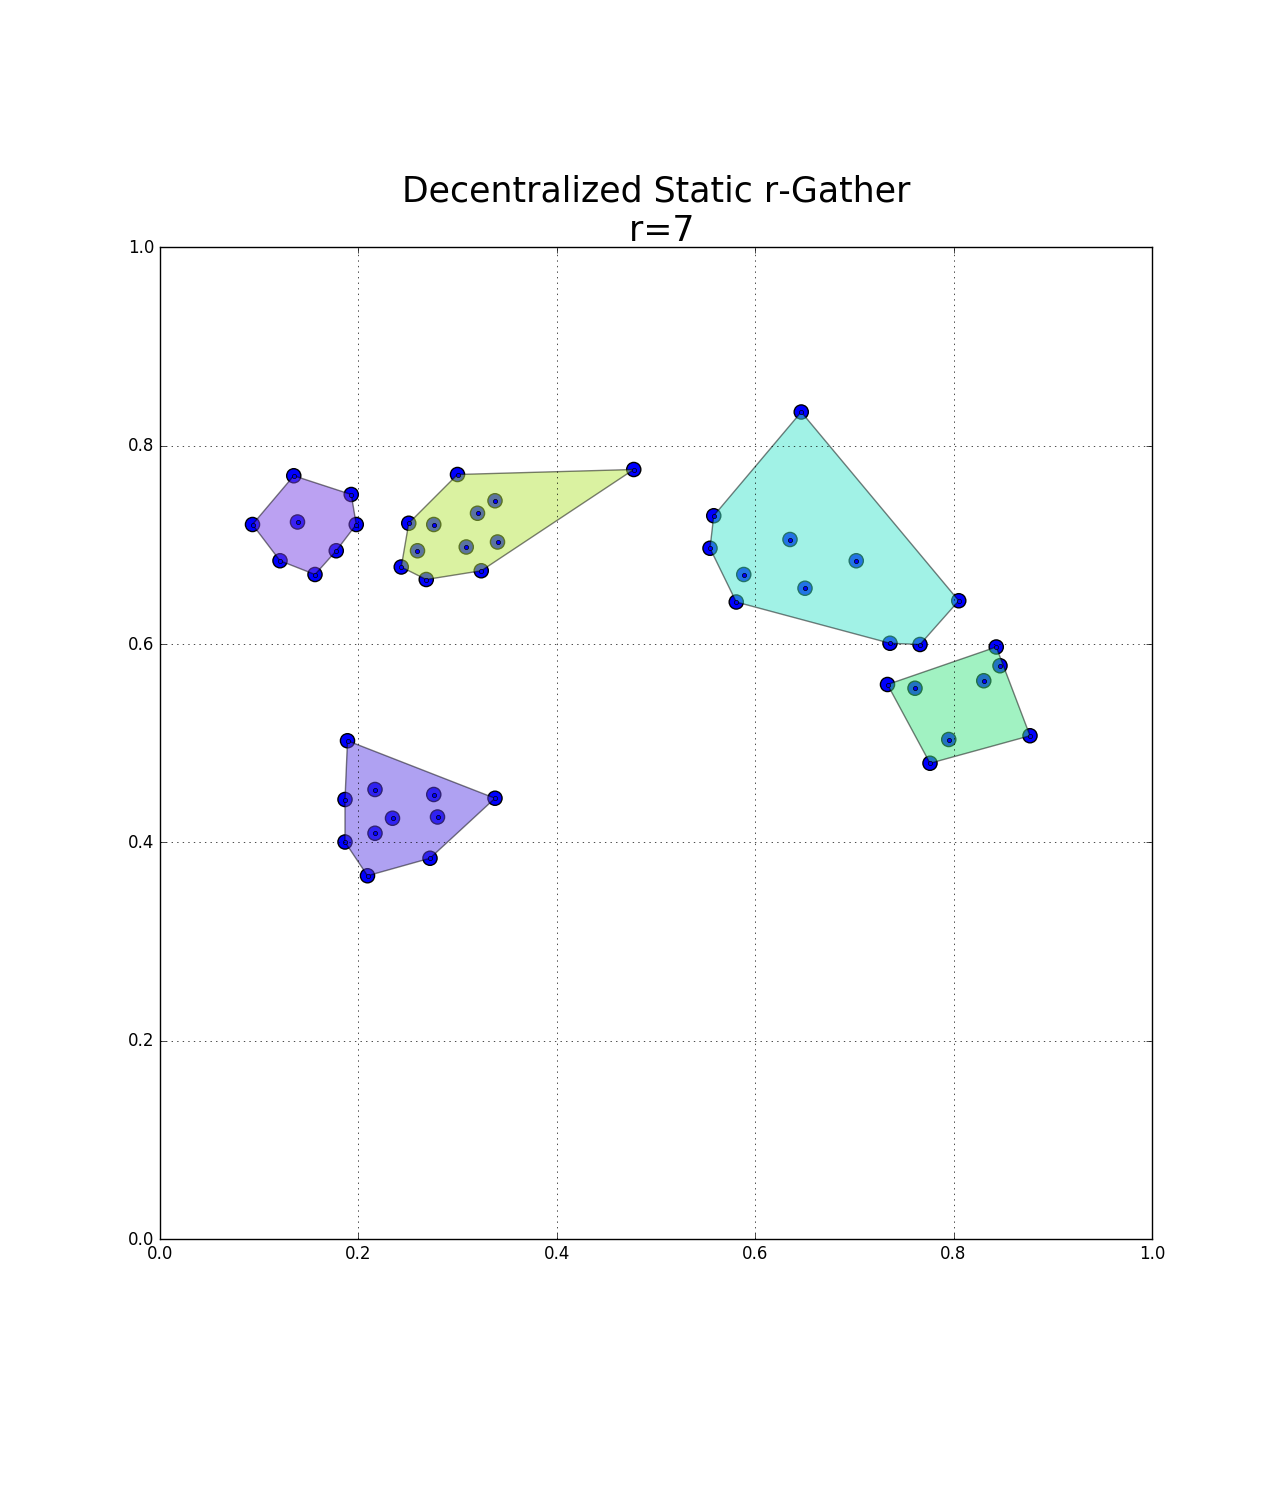
\includegraphics[scale=0.25]{figs/r7.png} & 
	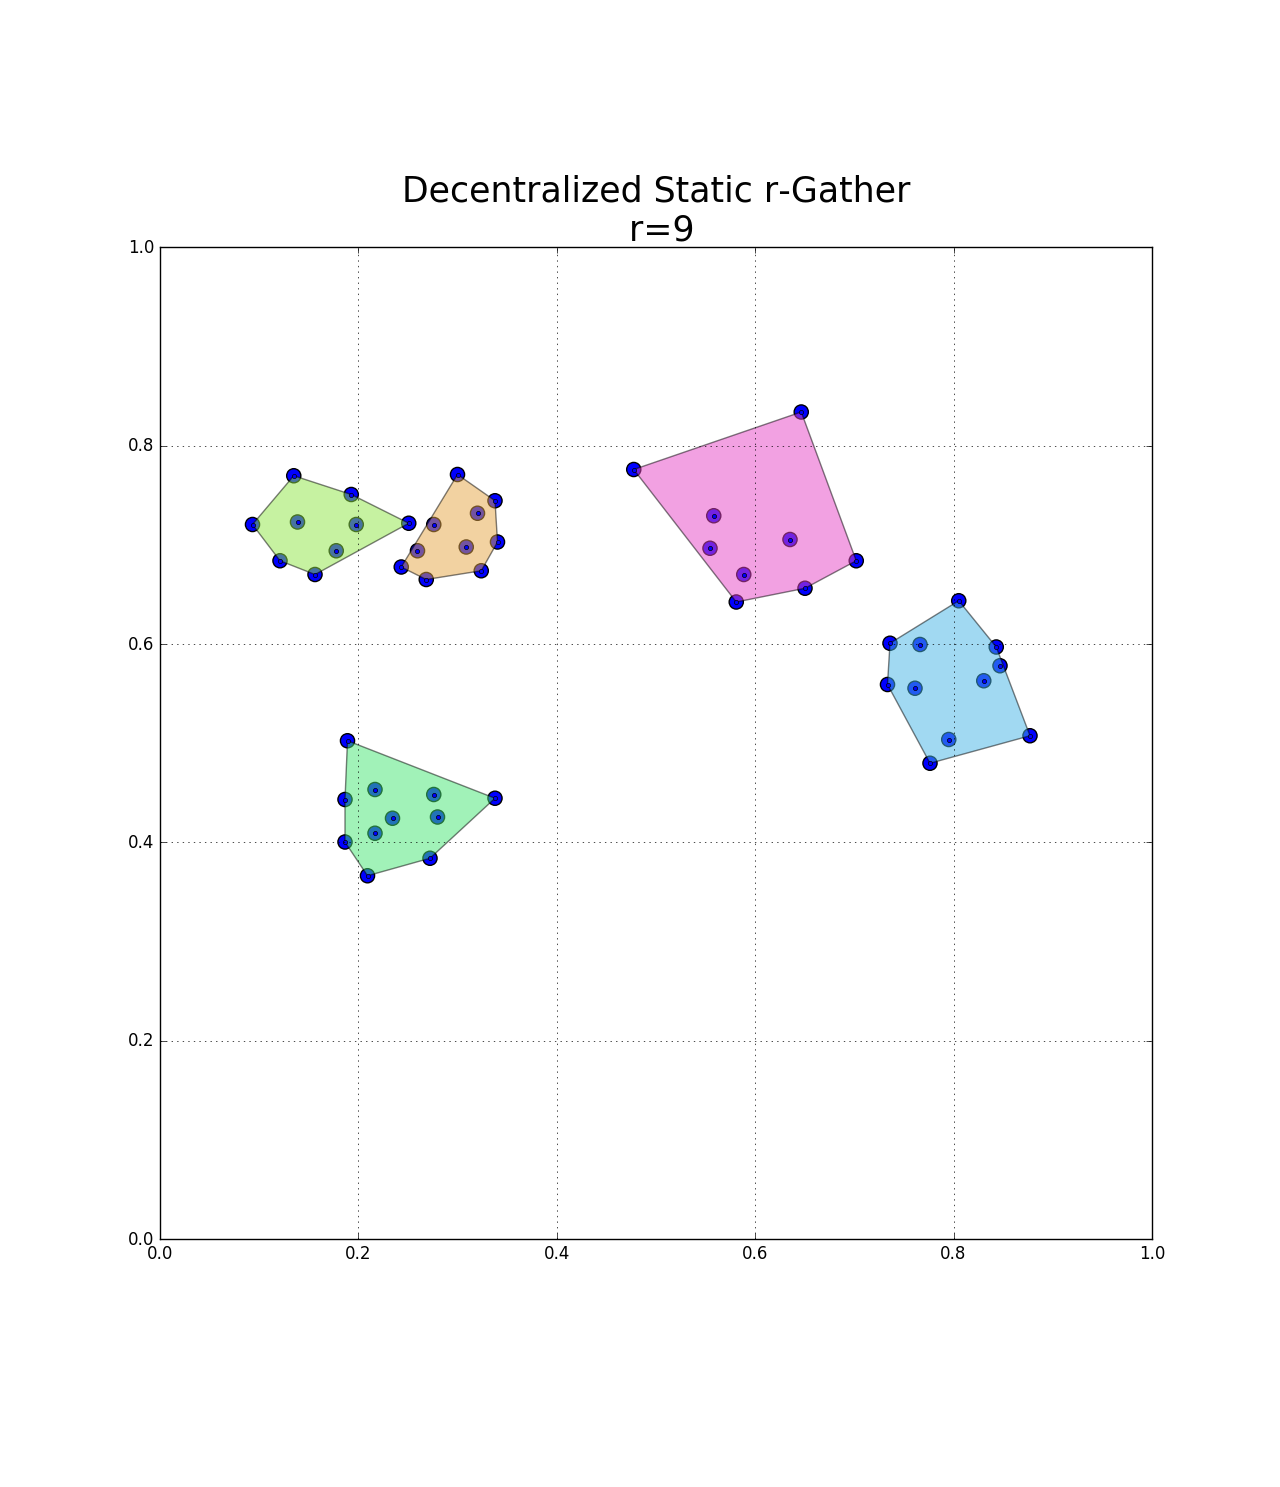
\includegraphics[scale=0.25]{figs/r9.png} 	\\
\vspace*{-6mm}
% \footnotesize (iii)& \footnotesize (iv) \\
\end{tabular}
\end{center}
%\vspace*{-6mm}
	\caption{\footnotesize The clusters produced by the distributed algorithm for a set of $50$ points randomly distributed, with $r=3$ in (top left), $r=5$ in (top right), $r=7$ in (bottom left) and $r=9$ in (bottom right) respectively. }
	\label{fig:snapshot}
%\vspace{-0.3in}
\end{figure*}

%\begin{figure}[h]
%\begin{center}
%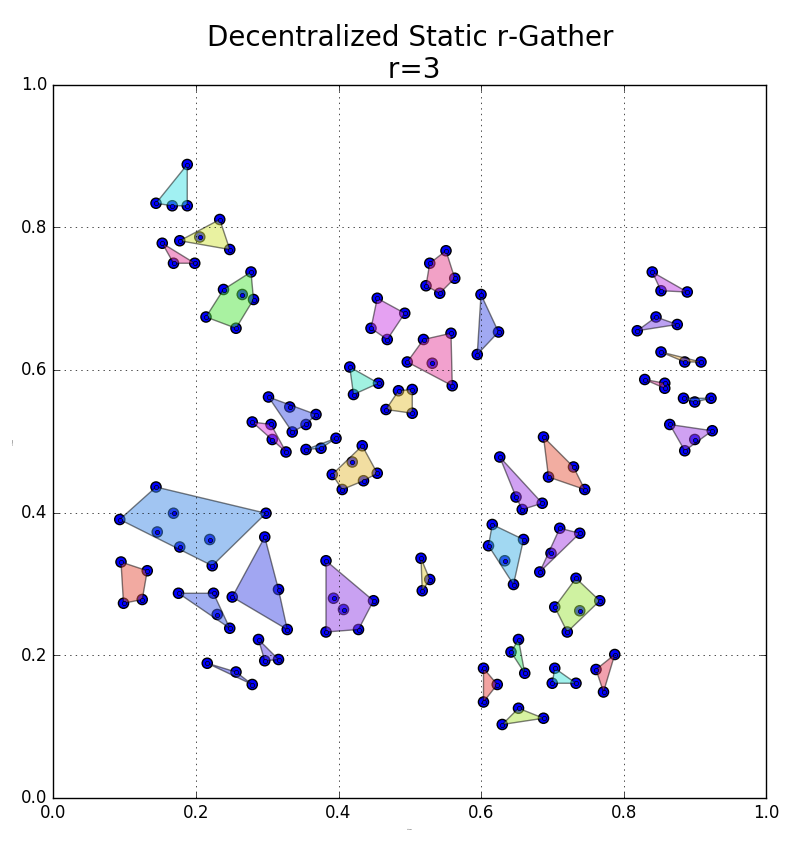
\includegraphics[width=3in]{figs/r3.png}
%\end{center}
%\end{figure}
%
%
%\begin{figure}[h]
%\begin{center}
%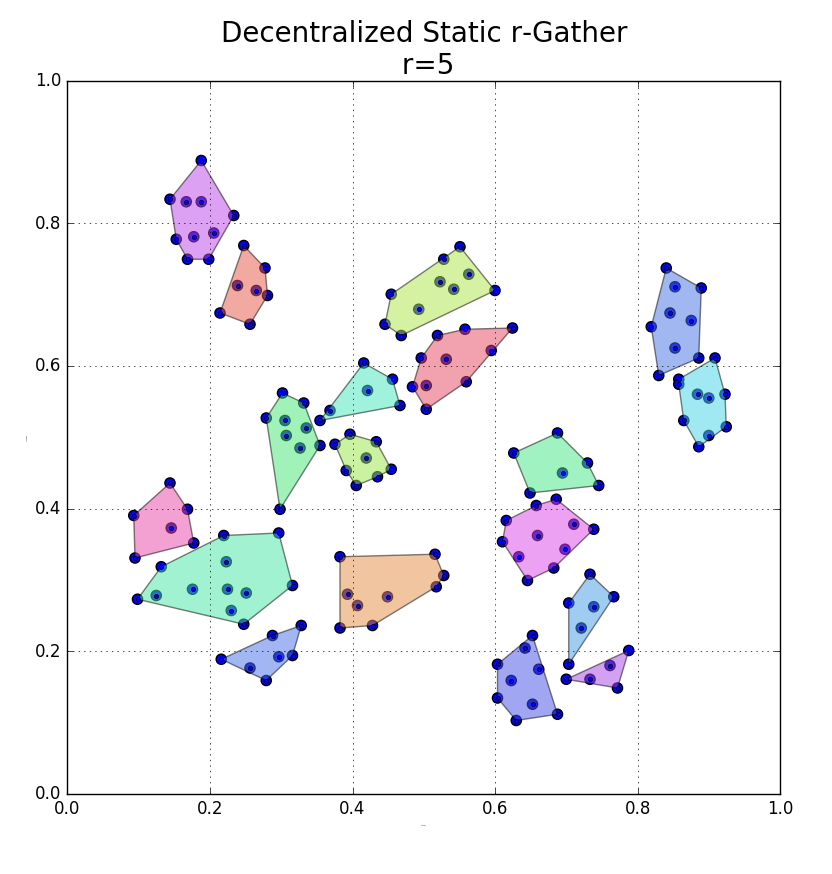
\includegraphics[width=3in]{figs/r5.png}
%\end{center}
%\end{figure}
%
%
%\begin{figure}[h]
%\begin{center}
%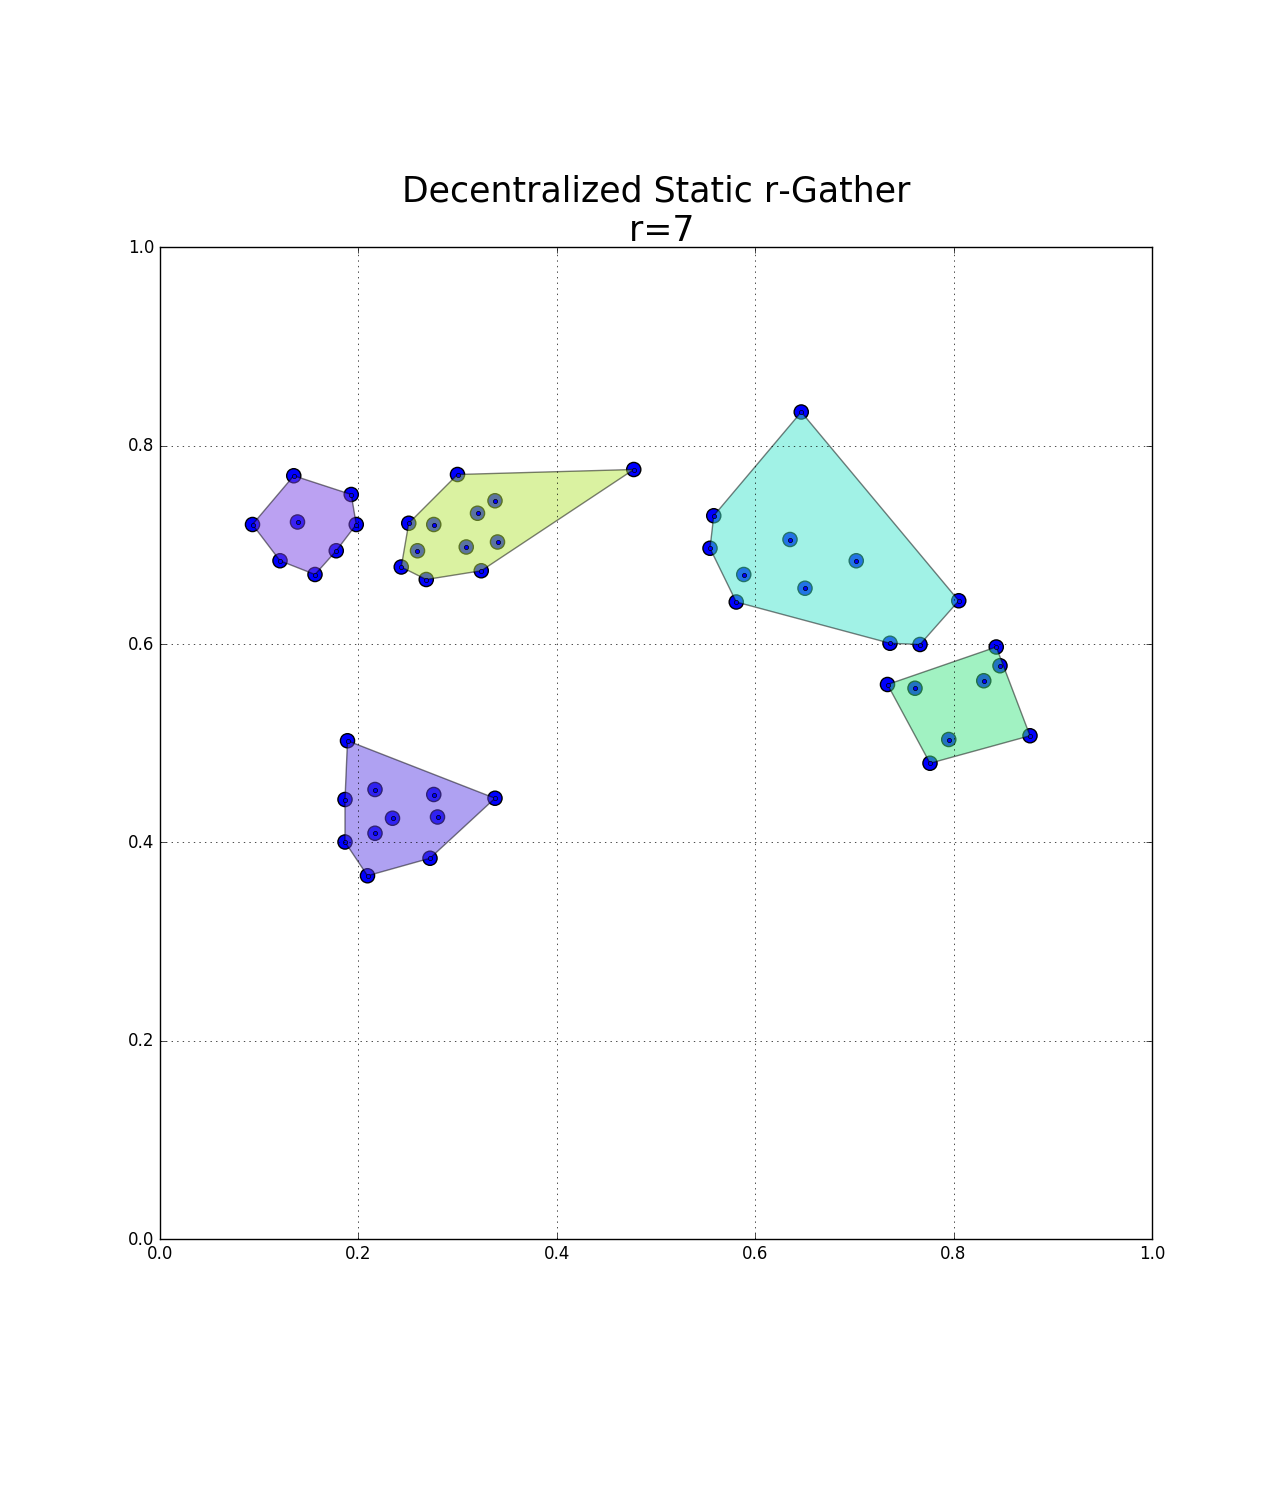
\includegraphics[width=3in]{figs/r7.png}
%\end{center}
%\end{figure}
%
%
%\begin{figure}[h]
%\begin{center}
%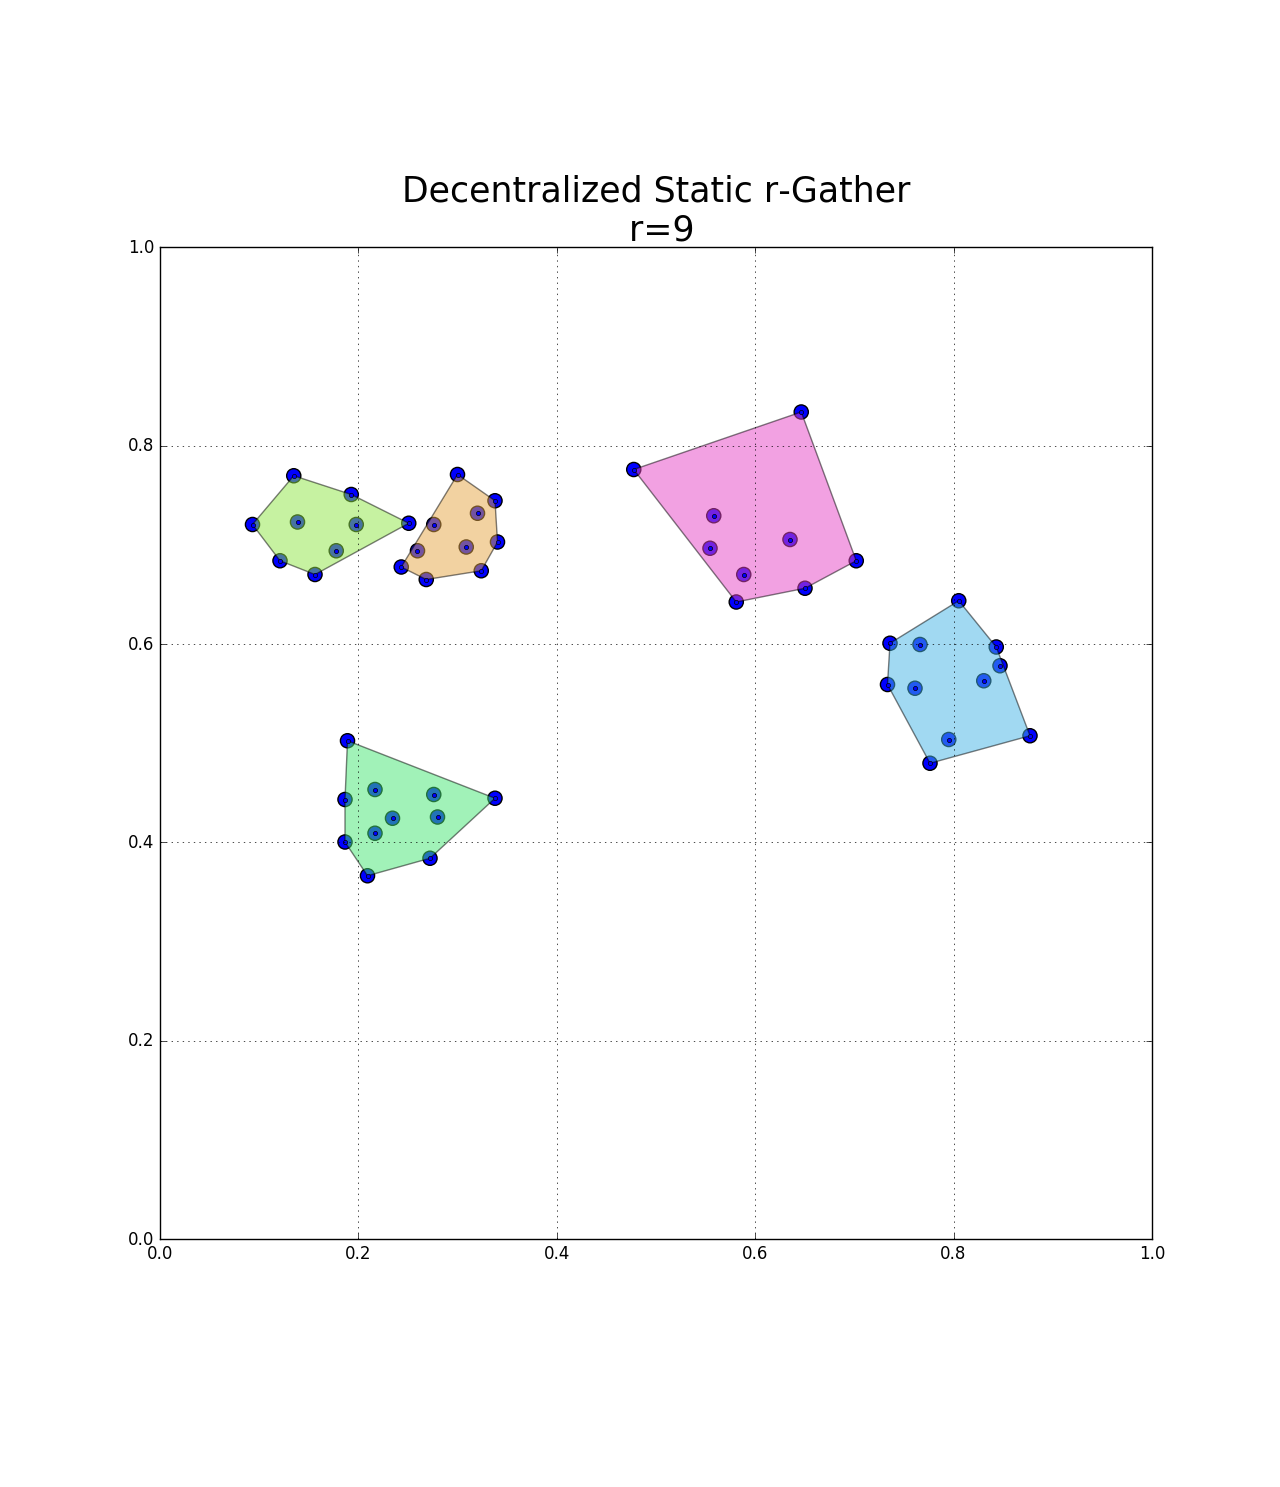
\includegraphics[width=3in]{figs/r9.png}
%\end{center}
%\end{figure}




%The $X$ and $Y$ axes in the figures above respectively denote longitude and latitude. 
%For generating these clusters and other experiments on the distributed algorithm to be described next, latitude and longitude pairs were treated simply as $x,y$ co-ordinates in $\mathbb{R}^2$. 

%\vspace{3mm}


%\subsection{Experiments}

%\vspace{3mm}


%\subsection{ Experimental Setup }        
%\vspace{2mm}


To test the quality of the clusterings generated for these algorithms for different $r$'s we calculated the maximum of the clusters' diameters. The distributed algorithm can be tweaked in several ways, such as finding a good maximal independent set of the $r$-neighborhoods of the nodes. In the first implementation, we calculate the distance from each node to the $r$th nearest neighbor. Then find the node $p$ which has the smallest such distance. Remove $p$ and its $r$-neighbors, repeat. In a different implementation, we just ran greedy maximal independent set and repeat $20$ times and take the best solution. 

We also plotted these statistics against the lower-bound $d_r^{\max}$, which is defined as follows. We take each node and calculate the distance to the $r$-th nearest neighbor, and take the maximum such value for all nodes. Clearly, any $r$-gather solution cannot have maximum diameter lower than $d_r^{\max}$.
For each clustering algorithm, we calculate the following two statistics:
\bitem
\item  The maximum over all clusters, the diameter of a cluster.  
\item  The $90$th percentile of the diameter of a cluster, over all clusters.
%\item  The  maximum over all clusters, the $90$th percentile of point-distances within a cluster.
\eitem

Further, we use a real data set including the GPS co-ordinates of $9386$ taxis in Shenzhen for a whole day, sampled at the interval of $5$ minutes. The average velocity is $14$ km/h.

Figure~\ref{fig:comparison} shows the performance of our algorithm in comparison
to~\cite{Aggarwal06achievinganonymity} and $d_{r}^{\max}$ as a baseline, on a snapshot containing $60$ random users from the dataset. Figure~\ref{fig:comparison-90} shows the $90\%$ percentile results.  

\begin{figure}[h]
\begin{center}
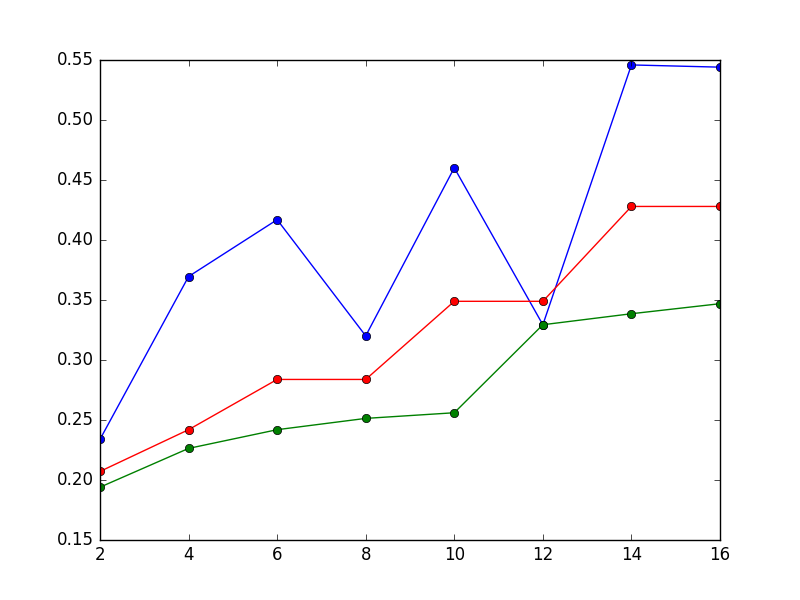
\includegraphics[width=3in]{figs/figure_1.png}
\caption{Max cluster diameter. Blue curve: approximation algorithm from~\cite{Aggarwal06achievinganonymity}; Red curve: distributed algorithm; Green curve: $d_{r}^{\max}$.}\label{fig:comparison}
\end{center}
\end{figure}


\begin{figure}[h]
\begin{center}
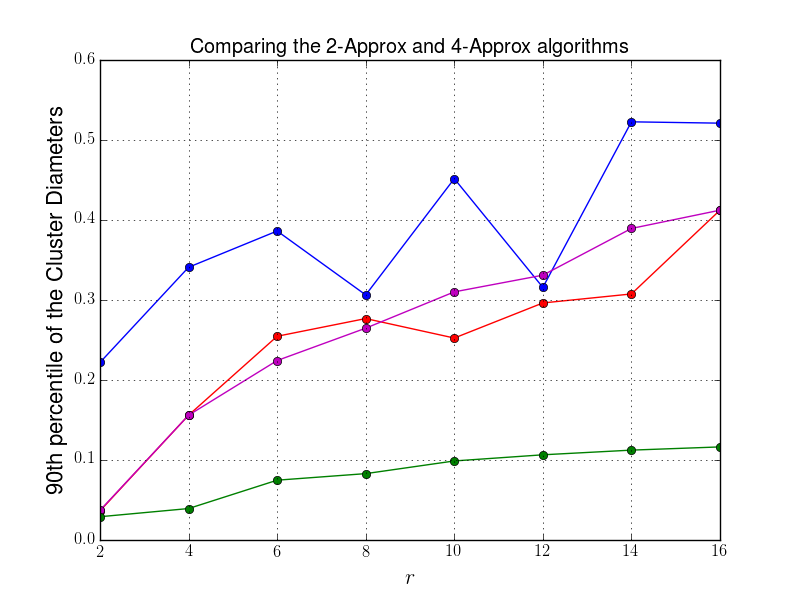
\includegraphics[width=3in]{figs/90thpercentile_60Cars.png}
\caption{$90\%$ percentile of all cluster diameter. Blue curve: approximation algorithm from~\cite{Aggarwal06achievinganonymity}; Red curve: distributed algorithm; Green curve: $d_{r}^{\max}$. Magenta: the distributed algorithm with the best maximal indepdenent set run over $20$ iterations.}\label{fig:comparison-90}
\end{center}
\end{figure}

Figure~\ref{fig:large} shows results on a larger dataset of $1500$
mobile users where the distributed still performs well. Figure~\ref{fig:large-90} shows the $90\%$ percentile results.  


\begin{figure}[h]
\begin{center}
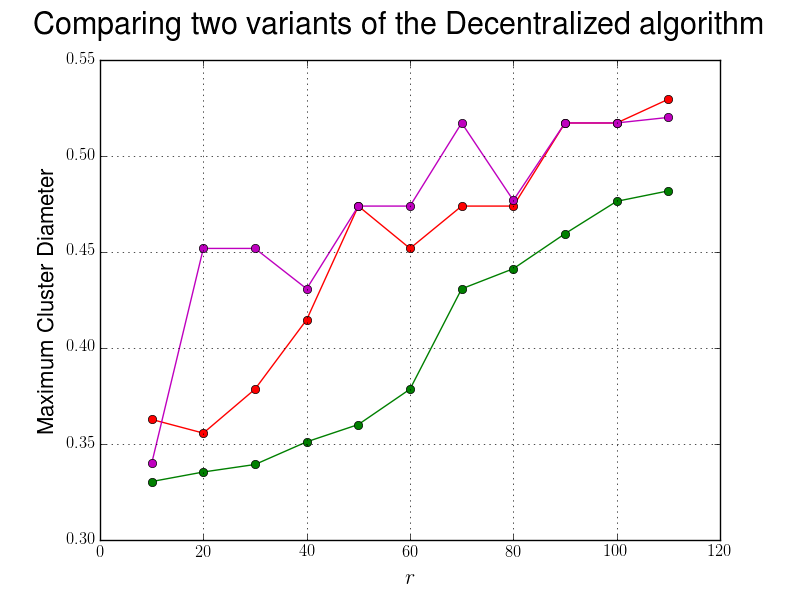
\includegraphics[width=3in]{figs/cars1500_4Approx.png}
\caption{Max cluster diameter on a snapshot of 1500 mobile users. Red curve: distributed algorithm; Green curve: $d_{r}^{\max}$. Magenta: the distributed algorithm with the best maximal indepdenent set run over $20$ iterations.}\label{fig:large}
\end{center}
\end{figure}

\begin{figure}[h]
\begin{center}
\includegraphics[width=3in]{figs/90thpercentile_1500cars.png}
\caption{$90\%$ percentile of all cluster diameter. 
Red curve: distributed algorithm; Green curve: $d_{r}^{\max}$. Magenta: the distributed algorithm with the best maximal indepdenent set run over $20$ iterations.}\label{fig:large-90}
\end{center}
\end{figure}

%\vspace{3mm}

%\bitem
%\item  The maximum over all clusters, the diameter of a cluster.  
%\item  The maximum over all clusters, the $90$th percentile of point-distances within a cluster.
%\eitem
%\vspace{3mm}

%\vspace{3mm}




%\vspace{20mm}




%We implemented the distributed algorithm and compared it with~ \cite{Aggarwal06achievinganonymity} and with the lower bound of $d_{r}^{\max}$  on real location data from a trajectory dataset of 9000 mobile users in Shenzen city in china. 

%
%\begin{figure}[h]
%\begin{center}
%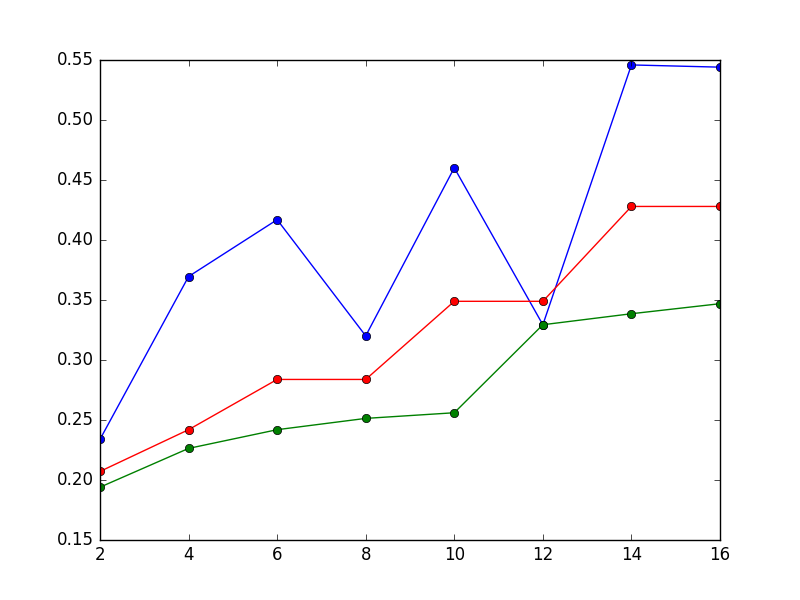
\includegraphics[width=3in]{figs/figure_1.png}
%\caption{Max cluster diameter. Black curve: approximation algorithm from~\cite{Aggarwal06achievinganonymity};
%  Red curve: distributed algorithm; Green curve: $d_{r}^{\max}$.}\label{fig:comparison}
%\end{center}
%\end{figure}






%We implemented the distributed algorithm and compared it with~\cite{Aggarwal06achievinganonymity} and with the lower bound of $d_{r}^{\max}$ on real location data from a trajectory dataset of 9000 mobile users in Shenzen city in china. 
Our main observations are:

\begin{itemize}
\item Our distributed algorithm usually produces better results than the $2$-approximation algorithm of~\cite{Aggarwal06achievinganonymity} in practice, although the approximation bound for the distributed algorithm is worse in theory.
\item The distributed algorithm runs faster and therefore can be run on larger datasets
\item The results (maximum cluster diameters) are close to the lower bound of $d_{r}^{\max}$.
\end{itemize}


%
%\begin{figure}[h]
%\begin{center}
%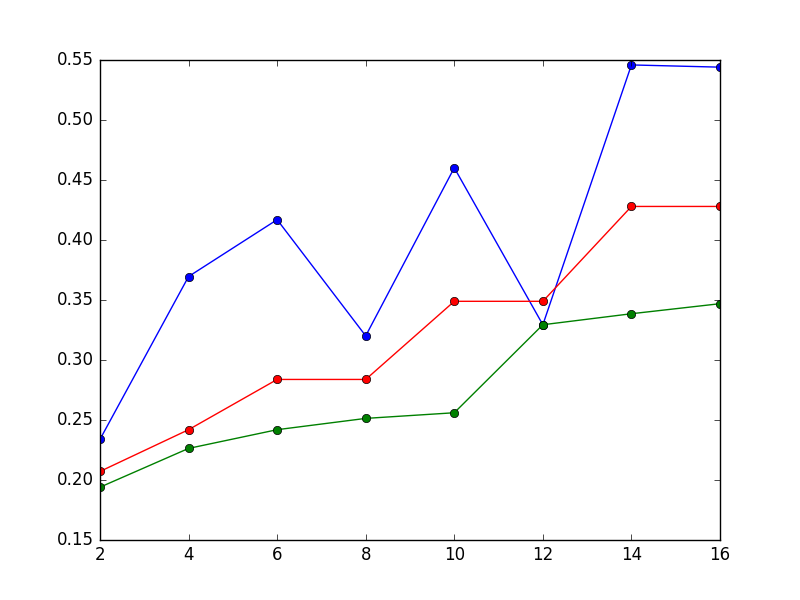
\includegraphics[width=3in]{figs/figure_1.png}
%\caption{Max cluster diameter. Black curve: approximation algorithm from~\cite{Aggarwal06achievinganonymity};
%  Red curve: distributed algorithm; Green curve: $d_{r}^{\max}$.}\label{fig:comparison}
%\end{center}
%\end{figure}

